\begin{enunciado}{20}
    There are a number of bounds on the generalization error $\epsilon$, all holding with probability at least $1 - \delta$.
    
    \letra{a} Original VC-bound:
    
    $$ \epsilon \le \sqrt{\frac{8}{N}\ln\frac{4m_{\hipotset}(2N)}{\delta}} $$
    
    \letra{b} Rademacher Penalty Bound:
    
    $$ \epsilon \le \sqrt{\frac{2\ln(2Nm_{\hipotset}(N))}{N}} + 
    \sqrt{\frac{2}{N}\ln\frac{1}{\delta}} + \frac{1}{N}$$
    
    \letra{c} Parrondo and Van den Broek:
    
    $$ \epsilon \le \sqrt{\frac{1}{N} \left( 2 \epsilon + \ln\frac{6m_{\hipotset}(2N)}{\delta} \right)} $$
    
    \letra{d} Devroye:
    
    $$ \epsilon \le \sqrt{\frac{1}{2N} \left( 4 \epsilon(1+\epsilon) + \ln\frac{4m_{\hipotset}(N^2)}{\delta} \right) } $$
    
    Note that (c) and (d) are implicit bounds in $\epsilon$. Fix $\dvc = 50$ and $\delta = 0.05$ and plot these bounds as a function of $N$. Which is best?
\end{enunciado}

O gráfico abaixo ilustra a variação do valor de $\epsilon$ de acordo com a quantidade de amostras (\emph(N)).

\begin{figure}[H]
    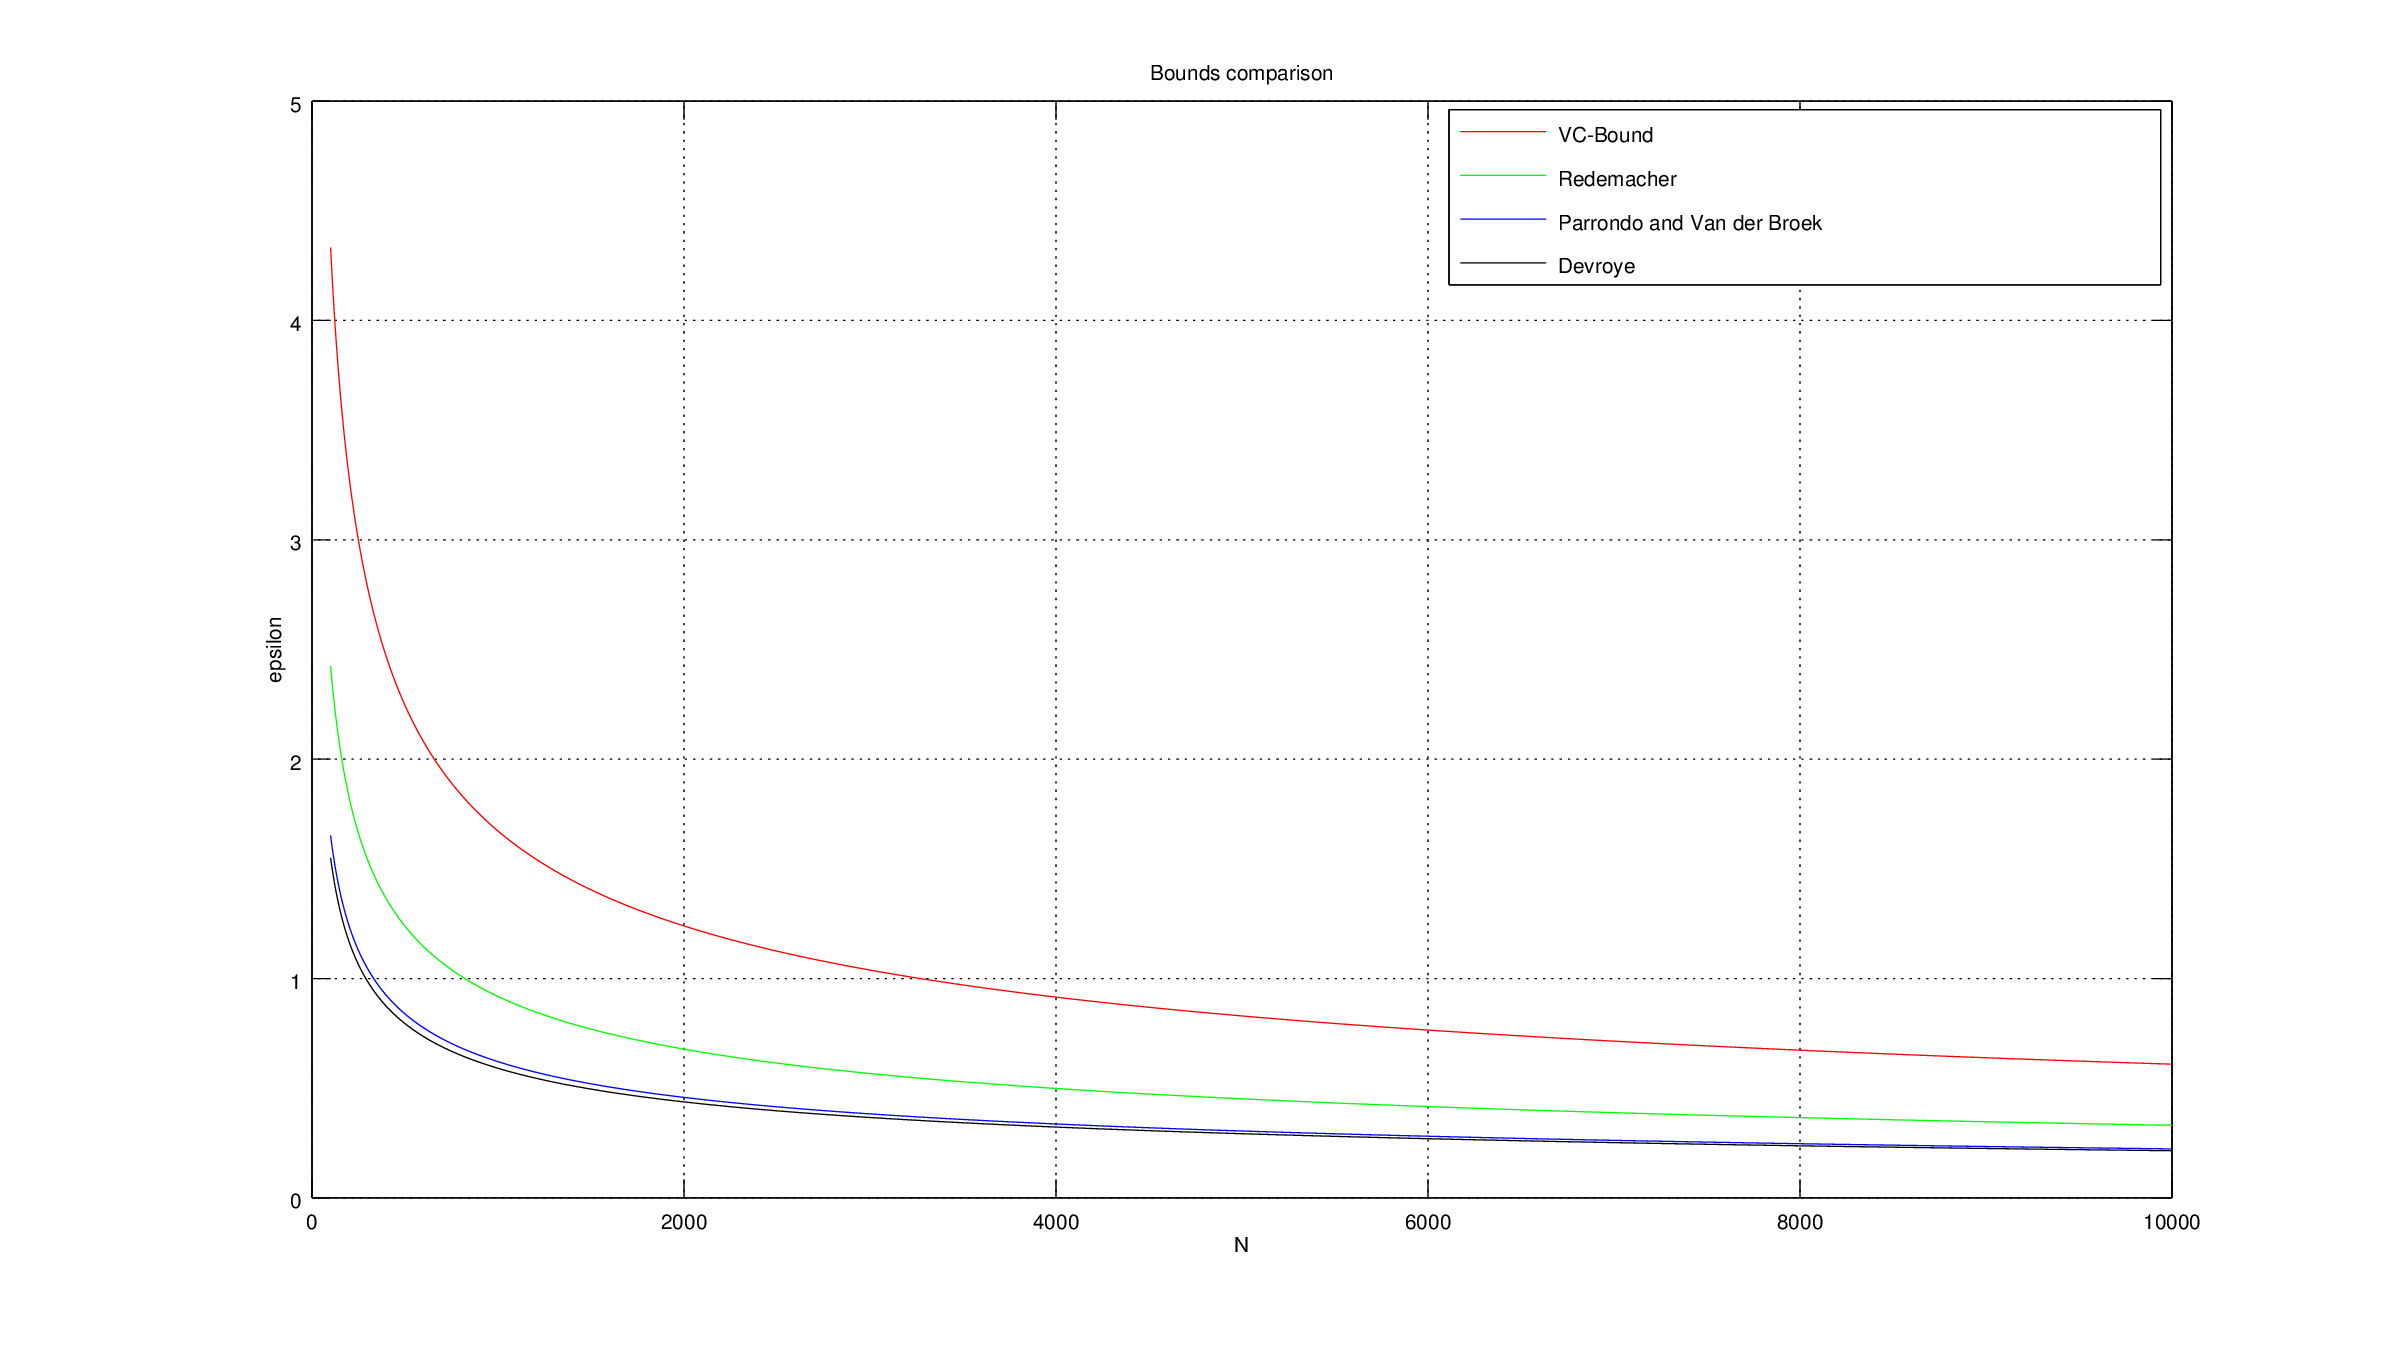
\includegraphics[width=\textwidth]{2-20.png}
    \caption{Comparação das condições de fronteira para o erro de generalização}
    \label{fig:f1}
\end{figure}

Sendo assim, podemos concluir que a melhor condição de fronteira é a de Devroye ( \letra{d}) pois, para obter uma dada precisão $\epsilon$, são necessárias menos amostras.  
